
%(BEGIN_QUESTION)
% Copyright 2009, Tony R. Kuphaldt, released under the Creative Commons Attribution License (v 1.0)
% This means you may do almost anything with this work of mine, so long as you give me proper credit

Read and outline the ``Progressive Valve Sequencing'' subsection of the ``Split-Ranging'' section of the ``Control Valves'' chapter in your {\it Lessons In Industrial Instrumentation} textbook.  Note the page numbers where important illustrations, photographs, equations, tables, and other relevant details are found.  Prepare to thoughtfully discuss with your instructor and classmates the concepts and examples explored in this reading.

\underbar{file i04221}
%(END_QUESTION)





%(BEGIN_ANSWER)


%(END_ANSWER)





%(BEGIN_NOTES)

Progressive split-ranging is when two control valves operate off the same signal, in such a way that one goes through its full range of motion before the other begins to move.  Useful for high-rangeability applications where no single valve size is adequate for all modes of operation -- one big valve would not handle low flows well, and one small valve would not be able to flow enough at the top end.  An automotive application of this is a progressively-staged carburetor, where one throttle butterfly opens up fully before the next begins to open.

\vskip 10pt

The following illustration graphically depicts this type of valve sequencing:

$$\includegraphics[width=15.5cm]{i04221x01.eps}$$




\vskip 20pt \vbox{\hrule \hbox{\strut \vrule{} {\bf Suggestions for Socratic discussion} \vrule} \hrule}

\begin{itemize}
\item{} Describe a practical application for {\it progressive} split-ranging.
\item{} Describe the progressive split-ranging used in certain {\it carburetors} in older automobile engines.
\end{itemize}







\vfil \eject

\noindent
{\bf Prep Quiz:}

Identify the style of valve sequencing represented by the following diagram:

$$\includegraphics[width=15.5cm]{i04221x01.eps}$$

\begin{itemize}
\item{} Exclusive
\vskip 5pt 
\item{} Complementary
\vskip 5pt 
\item{} Inclusive
\vskip 5pt 
\item{} Progressive
\vskip 5pt 
\item{} Gratuitous
\vskip 5pt 
\item{} Ostentatious
\end{itemize}


%INDEX% Reading assignment: Lessons In Industrial Instrumentation, split-ranging (progressive)

%(END_NOTES)


